\begin{lstlisting}
习题5.1第2,3,5,10,12,16题

习题5.4第2,4题
\end{lstlisting}
\begin{exercise}
\begin{figure}[H]
\centering
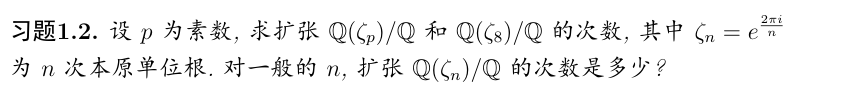
\includegraphics[width=\textwidth]{hw10-2025060116.png}
% \caption{}
\label{}
\end{figure}
\end{exercise}
Consider the cyclotomic polynomial
\[
\Phi _n(x)\coloneqq \prod_{a\in \mathbf{Z}^{\times}_n}(x-\zeta^{a}_n)
\]
\begin{figure}[H]
\centering
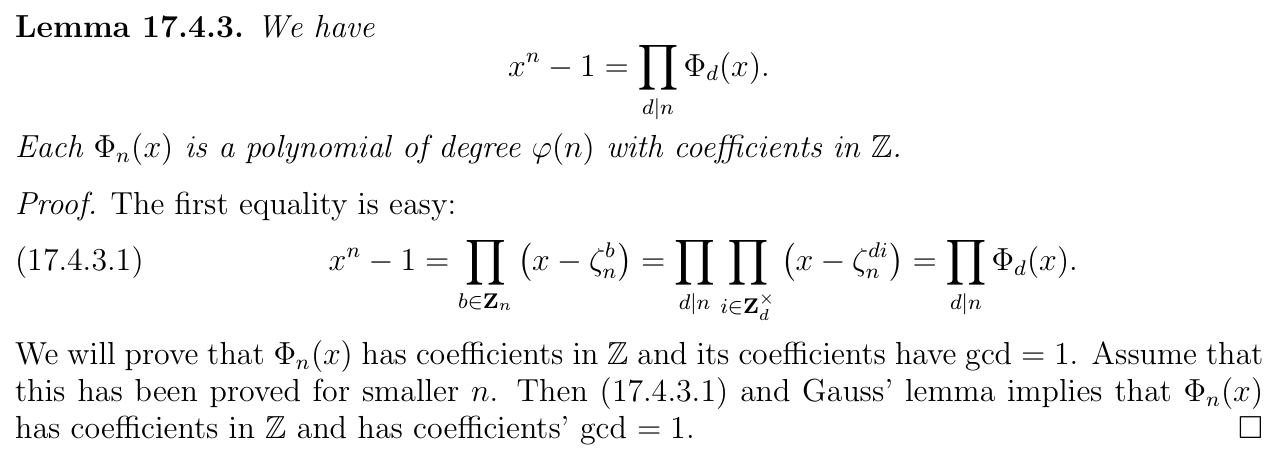
\includegraphics[width=\textwidth]{10-hw10-2025060116.png}
% \caption{}
\label{}
\end{figure}
\begin{figure}[H]
\centering
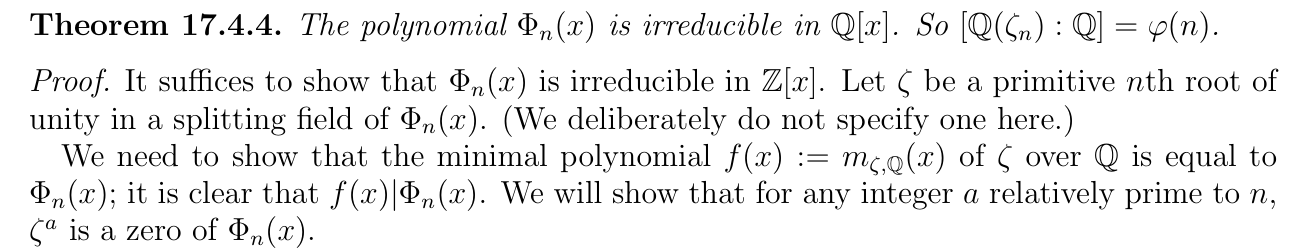
\includegraphics[width=\textwidth]{11-hw10-2025060116.png}
% \caption{}
\label{}
\end{figure}
\begin{figure}[H]
\centering
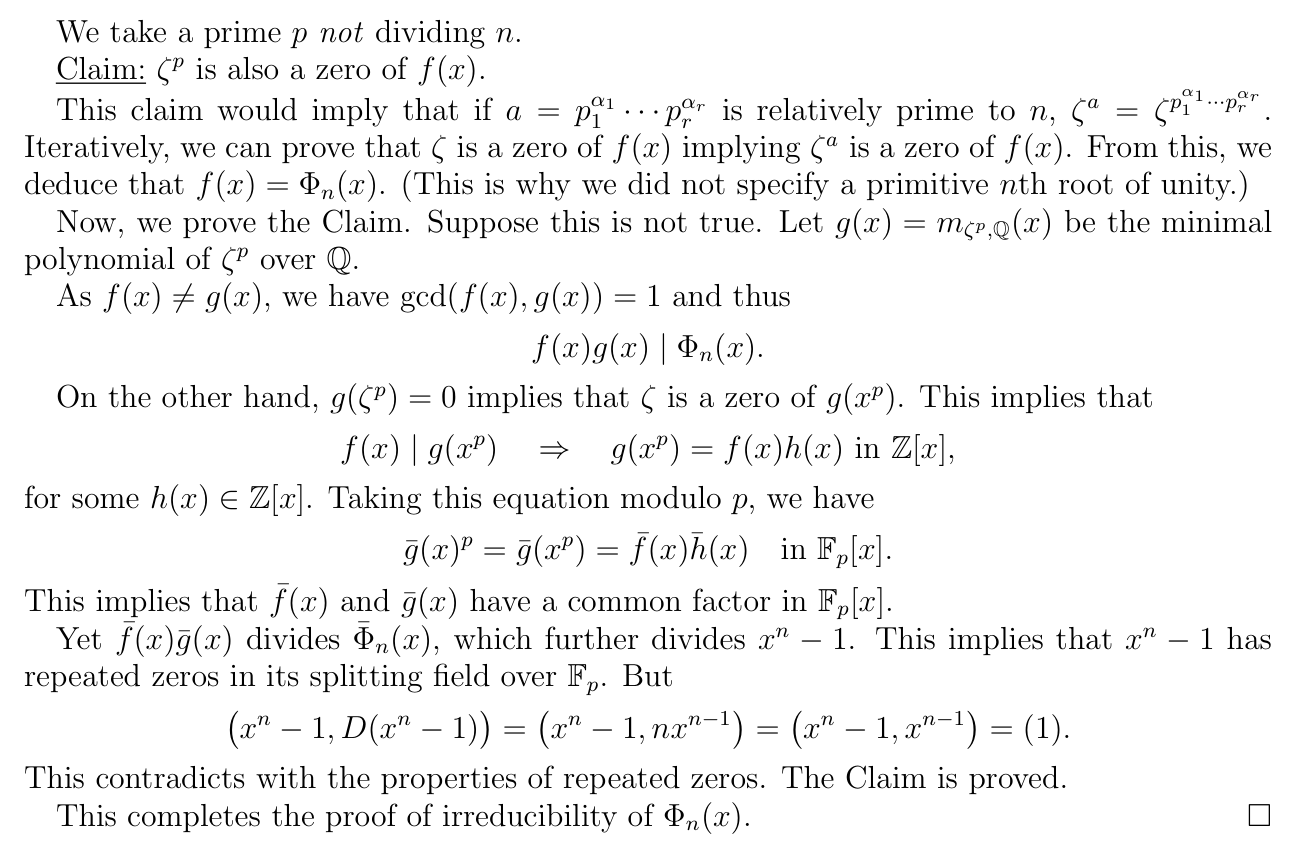
\includegraphics[width=\textwidth]{12-hw10-2025060116.png}
% \caption{}
\label{}
\end{figure}

\begin{exercise}
\begin{figure}[H]
\centering

\includegraphics[width=\textwidth]{1-hw10-2025060116.png}
% \caption{}
\label{}
\end{figure}
\end{exercise}
Let $x=\sqrt{ 2 }+\sqrt{ 3 }$, then
\[
\begin{aligned}
x & =\sqrt{ 2 }+\sqrt{ 3 } \\
x^2 & =5+2\sqrt{ 6 } \\
x^3 & =11 \sqrt{2}+9 \sqrt{3} \\
x^{4} & =20 \sqrt{6}+49
\end{aligned}
\]
(1) we know that $f(x)\coloneqq(x^2-5)^2-24=0$, and $f(x)=x^{4}-10x^2+1$ is irreducible over $\mathbb{Q}$ by Eisenstein criterion, thus is the minimal polynomial of $\sqrt{ 2 }+\sqrt{ 3 }$ over $\mathbb{Q}$.

(2) we know that $f(x)\coloneqq(x-\sqrt{ 2 })^2-3=0$ and $f(x)=x^2-2\sqrt{ 2 }x-1$ is of degree 2. The minimal polynomial cannot have degree 1 since $\sqrt{ 2 }+\sqrt{ 3 }\not\in \mathbb{Q}(\sqrt{ 2 })$, but divides $f(x)$, thus equals to $f(x)$ due to the uniqueness.

(3) we know that $f(x)\coloneqq x^2-5-2\sqrt{ 6 }=0$. Similar to the assertion in (2), $f(x)$ is the minimal polynomial of $\sqrt{ 2 }+\sqrt{ 3 }$ over $\mathbb{Q}(\sqrt{ 6 })$.

\begin{exercise}
\begin{figure}[H]
\centering

\includegraphics[width=\textwidth]{2-hw10-2025060116.png}
% \caption{}
\label{}
\end{figure}
\end{exercise}
For any $0\neq d\in D\subseteq F$, we have $f(d)=0$ for some $f\in K[x]$.
\[
f(x)=x^{n}+a_{n-1}x^{n-1}+\dots+a_0
\]
WLOG, assume that $a_0\neq0$, then
\[
d ^{-1}=-\underbrace{ a_0 ^{-1} }_{ \in K\subseteq D }(\underbrace{ d^{n-1}+a_{n-1}d^{n-2}+\dots+a_1 }_{ \in D })\in D
\]
Thus $D$ is field.

\begin{exercise}
\begin{figure}[H]
\centering
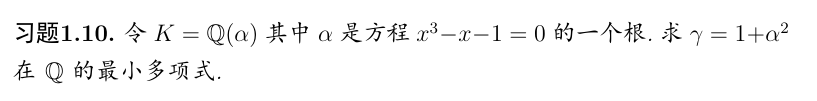
\includegraphics[width=\textwidth]{3-hw10-2025060116.png}
% \caption{}
\label{}
\end{figure}
\end{exercise}
\[
\begin{aligned}  
\gamma & =1+\alpha^{2} \\
\gamma^{2} & =3\alpha^{2}+\alpha+1 \\
\gamma^{3} & =7\alpha^{2}+5\alpha+2
\end{aligned}
\]
We have
\[
\gamma^{3}-5\gamma^{2}+8\gamma-5=0
\]
In $\mathbb{F}_{2}$, the polynomial
\[
\gamma^{3}-5\gamma^{2}+8\gamma-5\equiv \gamma^{3}+\gamma^{2}+1\mod2
\]
is irreducible. Then $\gamma^{3}-5\gamma^{2}+8\gamma-5$ is not reducible over $\mathbb{Q}$, thus the minimal polynomial of $\gamma$ over $\mathbb{Q}$ is
\[
x^3-5x^2+8x-5
\]
\begin{exercise}
\begin{figure}[H]
\centering

\includegraphics[width=\textwidth]{4-hw10-2025060116.png}
% \caption{}
\label{}
\end{figure}
\end{exercise}
(1)
\[
f(x)\coloneqq x^3-6x^2+9x+3
\]
is irreducible over $\mathbb{Q}$ by Eisenstein criterion, thus is the minimal polynomial of $u$ over $\mathbb{Q}$. By the definition of minimal polynomial,
\[
[\mathbb{Q}(u):\mathbb{Q}]=3
\]
(2)
We have
\[
u^3-6u^2+9u+3=0
\]
Then
\[
\begin{aligned}
u^{4} & =u(6u^2-9u-3) \\
 & =6u^3-9u^2-3u \\
 & =6(6u^2-9u-3)-9u^2-3u \\
 & =27u^2-57u-18
\end{aligned}
\]
We know that
\[
((u+1)-1)^3-6((u+1)-1)^2+9((u+1)-1)+3=0
\]
i.e.
\[
(u+1)^3-9(u+1)^2+24(u+1)-13=0
\]
Thus
\[
(u+1)^{-1}=\frac{1}{13}[(u+1)^2-9(u+1)+24]=\frac{u^2}{13}-\frac{7 u}{13}+\frac{16}{13}
\]
(3)
Suppose that
\[
(u^2-6u+8)^{-1}=au^2+bu+c
\]
Then
\[
(u^2-6u+8)(au^2+bu+c)=1
\]
i.e.
\[
\begin{aligned}
1 & =au^{4}+(b-6a)u^3+(8a+c-6)u^2+(8b-6c)u+8c \\
 & =au(6u^2-9u-3)+(b-6a)(6u^2-9u-3)+(8a+c-6)u^2+(8b-6c)u+8c \\
 & =(18a-3b+8c)+(51a-b-6c)u+(-6-37a+6b+c)u^2+6au^3 \\
 & =(18a-3b+8c)+(51a-b-6c)u+(-6-37a+6b+c)u^2+6a(6u^2-9u-3) \\
 & =(-3b+8c)+(-3a-b-6c)u+(-a+6b+c)u^2
\end{aligned}
\]
Let
\[
\begin{cases}
-3b+8c & =1 \\
-3a-b-6c & =0 \\
-a+6b+c & =0
\end{cases}
\]
Then
\[
(a,b,c)=\left( -\frac{35}{179},-\frac{9}{179},\frac{19}{179}    \right)
\]
Thus
\[
(u^2-6u+8)^{-1}=-\frac{35}{179}u^2-\frac{9}{179}u+\frac{19}{179} 
\]
\begin{exercise}
\begin{figure}[H]
\centering

\includegraphics[width=\textwidth]{7-hw10-2025060116.png}
% \caption{}
\label{}
\end{figure}
\end{exercise}
(1)
$1,u,u^2,\dots,u^{m-1}$ is the $K$ -basis for $F$, and $1,v,v^2,\dots,v^{n-1}$ is the $K$ -basis for $E$. Then
\[
FE=K(u,v)
\]
has elements of the form
\[
\sum_{\substack{i=0,1,\dots,m-1\\j=0,1,\dots,n-1}}a_{ij}u^{i}v^{j}
\]
From $FE=F(v)$, we see that $1, v, \dots,v^{n-1}$ span $FE$ over $F$. Hence $[FE:F]\leq n=[E:K]$ with equality iff these elements are linearly independent over $F$. Since $[FE:K]=[FE:F][F:K]$, we are done!

(2)
\[
m=[F:K]\mid [F:K]\cdot[FE:F]=[FE:K]
\]
\[
n=[E:K]\mid [FE:K]
\]
Since $(m,n)=1$, $mn \mid[FE:K]$. By (1), we have $[FE:K]\leq mn$. Thus
\[
[FE:K]=mn
\]
\begin{exercise}
\begin{figure}[H]
\centering

\includegraphics[width=\textwidth]{8-hw10-2025060116.png}
% \caption{}
\label{}
\end{figure}
\end{exercise}
$\mathbb{F}_{2}$ 上全部次数 $\leq4$ 的不可约多项式
\[
\begin{gathered}
x \\
x-1 \\
x^2+x+1 \\
x^3+x^2+1 \\
x^3+x+ 1 \\
x^{4}+x^3+1 \\
x^{4}+x^2+1 \\
x^{4}+x+1 \\
x^{4}+x^3+x^2+x+1
\end{gathered}
\]
$\mathbb{F}_{3}$ 上全部 2 次不可约多项式
\[
\begin{gathered}
x^2+1  \\
x^2+x+2 \\
x^2+2x+2 \\
2x^2+2 \\
2x^2+2x+1 \\
2x^2+x+1
\end{gathered}
\]
\begin{exercise}
\begin{figure}[H]
\centering

\includegraphics[width=\textwidth]{9-hw10-2025060116.png}
% \caption{}
\label{}
\end{figure}
\end{exercise}
Over $\mathbb{Q}$, denote $\gamma=\alpha_1+\alpha_2$, then
\[
\gamma^{2}=5+2\alpha_1\alpha_2
\]
Then
\[
(\gamma^{2}-5)^2=(2\alpha_1\alpha_2)^2=24
\]
i.e.
\[
\gamma^{4}-10\gamma^{2}+1=0
\]
On the other hand,
\[
[\mathbb{Q}(\alpha_1+\alpha_2):\mathbb{Q}]=\underbrace{ [\mathbb{Q}(\alpha_1+\alpha_2):\mathbb{Q}(\alpha_1)] }_{ =[\mathbb{Q}(\alpha_1)(\alpha_2):\mathbb{Q}(\alpha_1)] }[\mathbb{Q}(\alpha_1):\mathbb{Q}]\overset{ ? }{ = }2\cdot2=4
\]
We just need to show that $\alpha_2 \not\in \mathbb{Q}(\alpha_1)$. Assume that $\alpha_2\in \mathbb{Q}(\alpha_1)$, then $\alpha_2=a+b\alpha_1$ for some $a, b\in \mathbb{Q}$, then
\[
3=\alpha_2^2=a^2+2b^2+2ab\alpha_1
\]
Then $\alpha_1=\frac{3-a^2-2b^2}{2ab}\in \mathbb{Q}$, if $ab\neq0$. Thus $3=\left( \frac{p}{q} \right)^2$ for some $p, q\in \mathbb{Z}$. Then
\[
3q^2=p^2
\]
The order of 3 in $3q^2$ is odd while in $p^2$ is even, which is a contradiction.

Therefore, $ab=0$. $b\neq0$ since $\alpha_2 \not\in \mathbb{Q}$ by the same discussion. $a\neq0$, otherwise $\alpha_2=b\alpha_1$ for some $b=\frac{p}{q}\in \mathbb{Q}$, where $p, q\in \mathbb{Z}$. Thus
\[
3=\frac{2p^2}{q^2}\implies 3q^2=2p^2
\]
which is absurd. Therefore $\alpha_2 \not\in \mathbb{Q}(\alpha_1)$.

As the minimal polynomial is unique, $m_{\gamma,\mathbb{Q}}(x)=x^{4}-10x^2+1$.

Over $\mathbb{F}_{5}$,
\[
x^{4}-10x^2+1\equiv x^{4}+1\mod 5
\]
Then $m_{\gamma,\mathbb{F}_{5}}(x)\mid x^{4}+1=(x^2+2)(x^2+3)$ in $\mathbb{F}_{5}$. Since $\alpha_1,\alpha_2 \not\in \mathbb{F}_{5}$, $m_{\gamma,\mathbb{F}_{5}}(x)$ is nontrivial. Thus $m_{\gamma,\mathbb{F}_{5}}(x)$ is either $x^2+2$ or $x^2+3$.
\[
\gamma^{2}+2=2+2\alpha_1\alpha_2
\]
\[
\gamma^{2}+3=3+2\alpha_1\alpha_2
\]
Then we assert that $2\alpha_1\alpha_2\in \mathbb{F}_{5}$ thus $\alpha_1\alpha_2\in \mathbb{F}_{5}$. As $(\alpha_1\alpha_2)^2=\alpha_1^2\alpha_2^2=2\cdot3=1$, we know that $\alpha_1\alpha_2=1\text{ or }4$.

If $\alpha_1\alpha_2=1$, then
\[
\gamma^{2}+2=(\alpha_1+\alpha_2)^2+2=2+2\alpha_1\alpha_2=4
\]
\[
\gamma^{2}+3=3+2\alpha_1\alpha_2=0
\]
$m_{\gamma,\mathbb{F}_{5}}=x^2+3$.

If $\alpha_1\alpha_2=4$, then
\[
\gamma^{2}+2=(\alpha_1+\alpha_2)^2+2=2+2\alpha_1\alpha_2=0
\]
\[
\gamma^{2}+3=3+2\alpha_1\alpha_2=1
\]
$m_{\gamma,\mathbb{F}_{5}}(x)=x^2+2$.

Over $\mathbb{F}_{7}$,
\[
x^{4}-10x^2+1\equiv x^{4}+4x^2+1\mod 7
\]
Then $m_{\gamma,\mathbb{F}_{7}}(x)\mid x^{4}+4x^2+1=(x^2+x+6)(x^2+6x+6)$. $m_{\gamma,\mathbb{F}_{7}}(x)$ is either $x^2+x+6$ or $x^2+6x+6$.
\[
\gamma^{2}+\gamma+6=4+2\alpha_1\alpha_2+\alpha_1+\alpha_2
\]
\[
\gamma^{2}+6\gamma+6=4+2\alpha_1\alpha_2+6\alpha_1+6\alpha_2
\]
Since $\alpha_1^2=2$, we have $\alpha_1=3\text{ or }4$.

If $\alpha_1=3$,
\[
\gamma^{2}+\gamma+6=4+6\alpha_2+3+\alpha_2=0
\]
Then $m_{\gamma,\mathbb{F}_{7}}(x)=x^2+x+6$.

If $\alpha_1=4$,
\[
\gamma^{2}+6\gamma+6=4+8\alpha_2+24+6\alpha_2=0
\]
Then $m_{\gamma,\mathbb{F}_{7}}(x)=x^2+6x+6$.
